%% Document template source: LaTeX2e template for FEUP's Project FE-UP
%% Document template author: jlopes@fe.up.pt
%% Template adapted

\documentclass[11pt,a4paper]{report}

%% Macros ----------------------------------------------------------------------{{{1
\newcommand{\school}{Instituto Superior de Engenharia de Lisboa}
\newcommand{\degree}{Licenciatura em Engenharia Eletrotécnica, Telecomunicações e Computadores}
%\newcommand{\projfeup}{Projeto FEUP 2023/24 --- LEIC}
\newcommand{\projtitle}{Título do Trabalho}
\newcommand{\projsubtitle}{Subtítulo do Trabalho}
\newcommand{\projteam}{Grupo 7}

%% Package ---------------------------------------------------------------------{{{1
\usepackage{graphicx}           % 
\usepackage[portuguese]{babel}  % [portuges]??
\usepackage{multicol}           % 
\usepackage{longtable}          % Tables continue in the next page
\usepackage{listings}           % Programming syntax

\usepackage[utf8]{inputenc}     % accents
\usepackage{color}


%% Package settings ------------------------------------------------------------{{{1
\graphicspath{{./images/}}                          % {graphicx} - Images path
\selectlanguage{portuguese}                         % {babel} - Language portuguese
\setlength{\columnsep}{3cm}                         % {multicol} - Column spacement
\definecolor{engineering}{rgb}{0.549,0.176,0.098}   % {color}
\definecolor{cloudwhite}{cmyk}{0,0,0,0.025}         % {color}
\lstdefinestyle{pythoncode}                         % {listings} - Python syntax
{
    keepspaces=true,
    numbersep=5pt,

    basicstyle=\footnotesize\ttfamily,
    keywordstyle=\bfseries,
    numbers=left,                      % where to put the line-numbers
    numberstyle=\scriptsize\texttt,    % the size of the fonts that are used for the line-numbers
    stepnumber=1,                      % the step between two line-numbers. If it's 1 each line will be numbered
    numbersep=8pt,                     % how far the line-numbers are from the code
    frame=tb,
    float=htb,
    aboveskip=8mm,
    belowskip=4mm,
    backgroundcolor=\color{cloudwhite},
    showspaces=false,                  % show spaces adding particular underscores
    showstringspaces=false,            % underline spaces within strings
    showtabs=false,                    % show tabs within strings adding particular underscores
    tabsize=2,                         % sets default tabsize to 2 spaces
    captionpos=b,                      % sets the caption-position to bottom
    breaklines=true,                   % sets automatic line breaking
    breakatwhitespace=false,           % sets if automatic breaks should only happen at whitespace
    escapeinside={\%*}{*)},            % if you want to add a comment within your code
    morekeywords={*,var,template,new}  % if you want to add more keywords to the set
}

%\usepackage{comment}               % Permite criar um segmento de comentários (/begin{comment} [...] /end{comment})
%\usepackage{xcolor}                % Colorir texto (esta versão é mais flexível do que a {color})
%\usepackage{subcaption}            % Subcaptions para figuras
%\usepackage{fullpage}              % Utilizar página inteira

%% Document start --------------------------------------------------------------{{{1
\begin{document}


%% Cover -----------------------------------------------------------------------{{{1

%% TOC -------------------------------------------------------------------------{{{1
\tableofcontents

%% List of figures -------------------------------------------------------------{{{1

%% List of tables --------------------------------------------------------------{{{1

%% Acronyms --------------------------------------------------------------------{{{1

%% Glossary --------------------------------------------------------------------{{{1

%% Chapter: introduction -------------------------------------------------------{{{1
\chapter{Introduction}
    Milestones:
    \begin{itemize}
        \item Getting apache2 web server running in localhost
        \item Access web server - http://127.0.0.1/
        \item Access web server from other computer
        \item Use wireshark to capture the web access from another host
        \item Compare the HTTP headers sent by the client and the server
        \item Develop a web client
        \item Establish a TCP connection to the server
        \item Request the base webpage
    \end{itemize}
    
    Web client requirements:
    \begin{itemize}
        \item Usage of HTTP library forbidden
        \item Establish TCP connection using available sockets library - send the HTTP request and receive the HTTP reply
        \item HTTP reply should be presented to the user
        \item - Optional - act to the various HTTP replies
        \item Text-only application
    \end{itemize}

%% Chapter: project ------------------------------------------------------------{{{1
\section{Project}
    \subsection{Software}
        local server:
            windows 11 x64
            xampp-portable-windows-x64-8.2.12-0-VS16.7z
        client:
            firefox version
            librefox version
            wireshark version
    
    \subsection{Configurations}
        SSLEngine disabled in apache to ease access with http
        %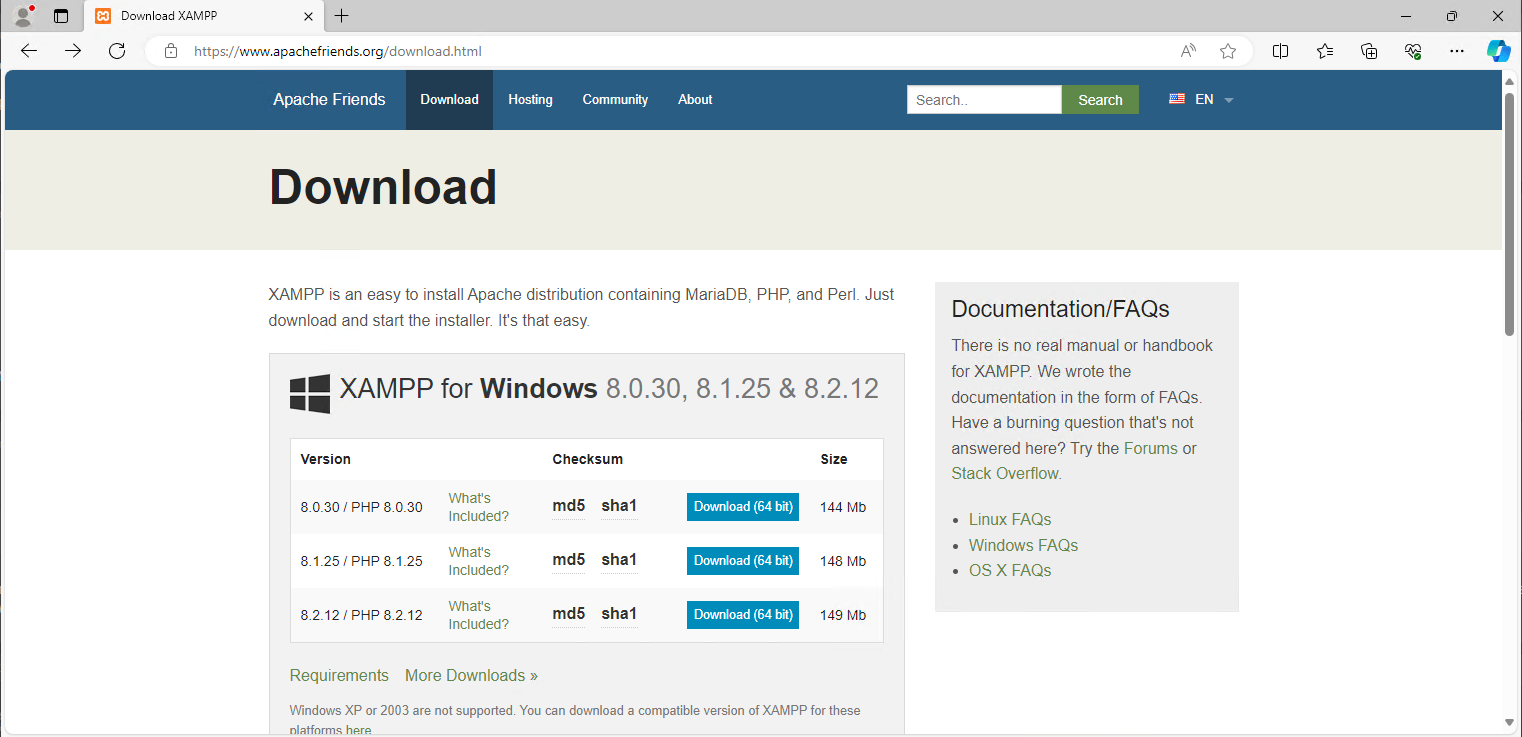
\includegraphics[scale=1.0]{xampp01} \\
        %<=++figure sslengine off++=>
        %<=++figure access from localhost++=>
        %<=++figure access from 127.0.0.1++=>
        %<=++figure access from anotherhost++=>
        %<=++figure wireshark capture from another host++=>
    
    \subsection{Python code}
        \lstset{style=pythoncode}
        \lstinputlisting[language=python, caption=Simple HTTP webclient using sockets in python]{webclient/httpsocketv3.py}
        The code was adapted to be simple and cycle through the various responses.
        Modifiable variables include serverName, serverPort and the httpTestMessages list.
        The httpTestMessages is built in a way that only the first part is necessary to modify.
    
    \subsection{List of headers}
        client
            meaning
        server
            meaning
    
    \subsection{Objectives}
        Step-by-step instructions performed
        Xampp install
        wireshark install
        wireshark settings
        wireshark filters
        
        \begin{tabular}{ l r }
            text & 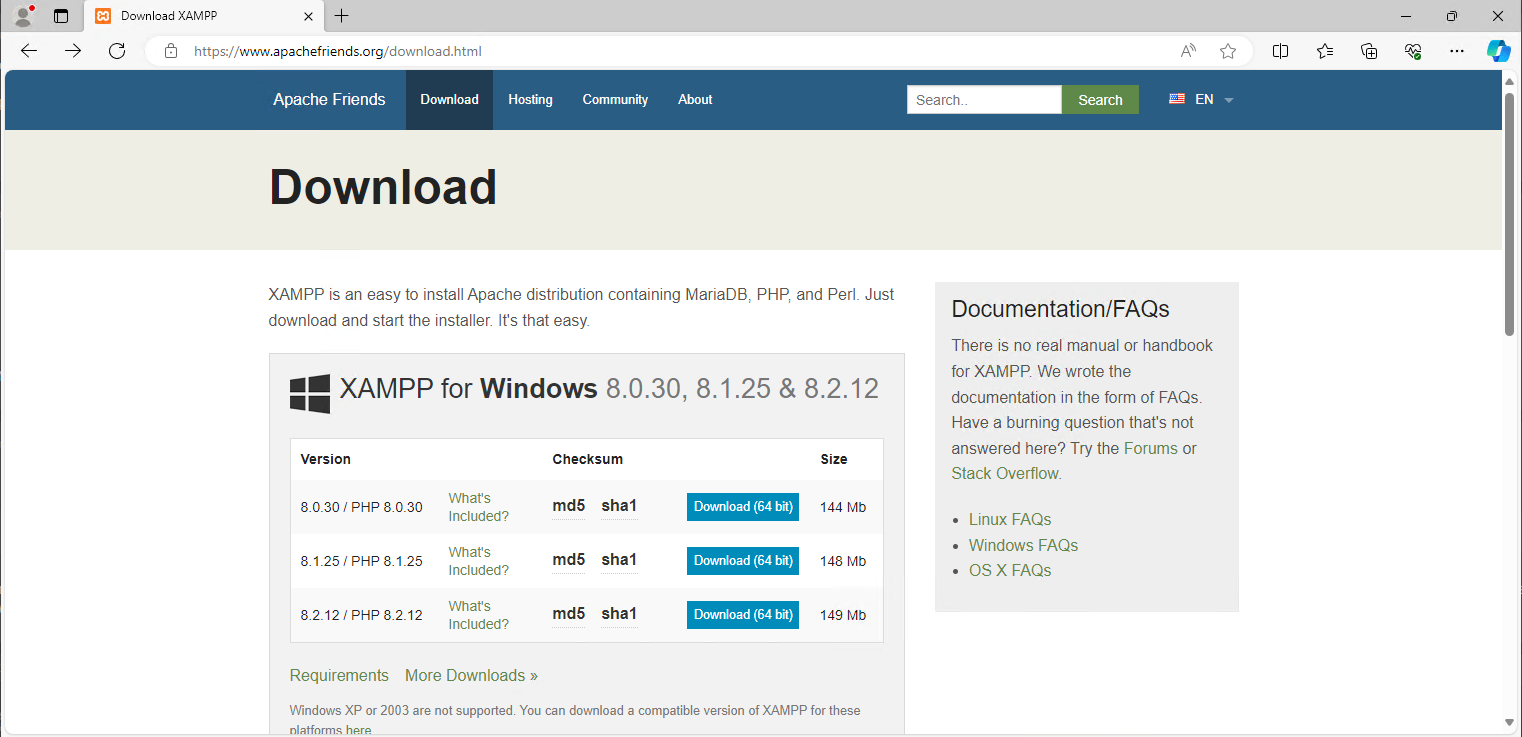
\includegraphics[scale=1.0]{xampp01} \\ % 0.3 scale!
            text & 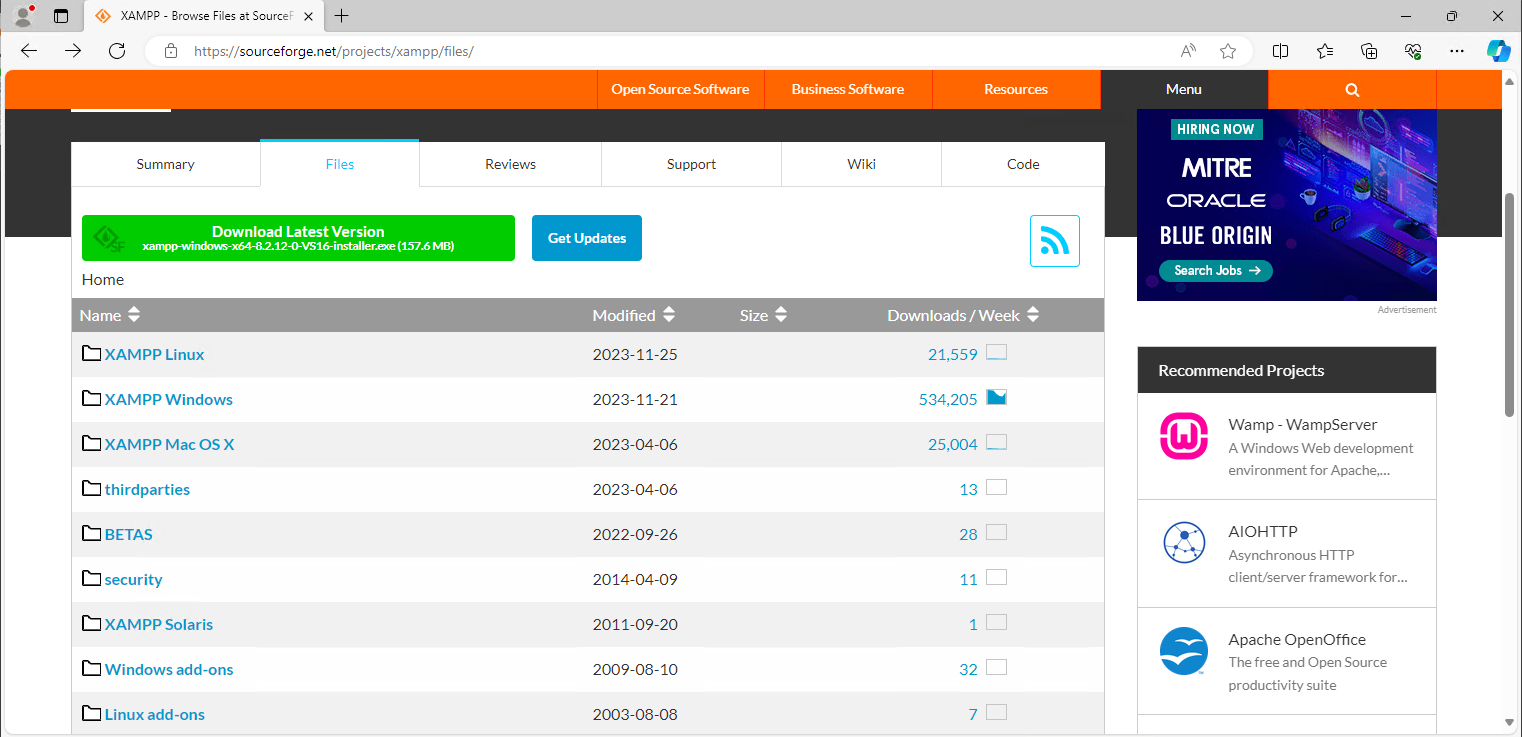
\includegraphics[scale=1.0]{xampp02} \\
            text & 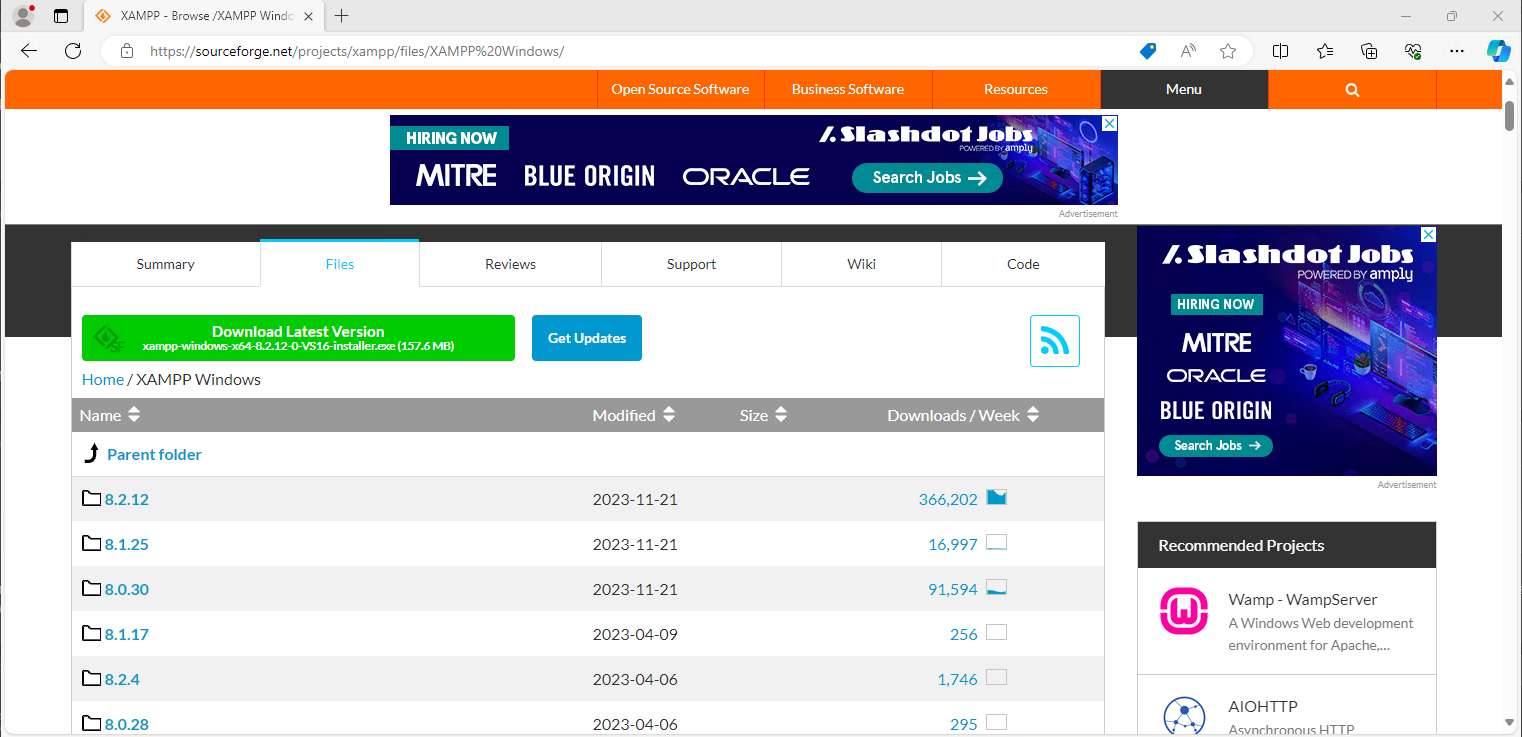
\includegraphics[scale=1.0]{xampp03} \\
            text & 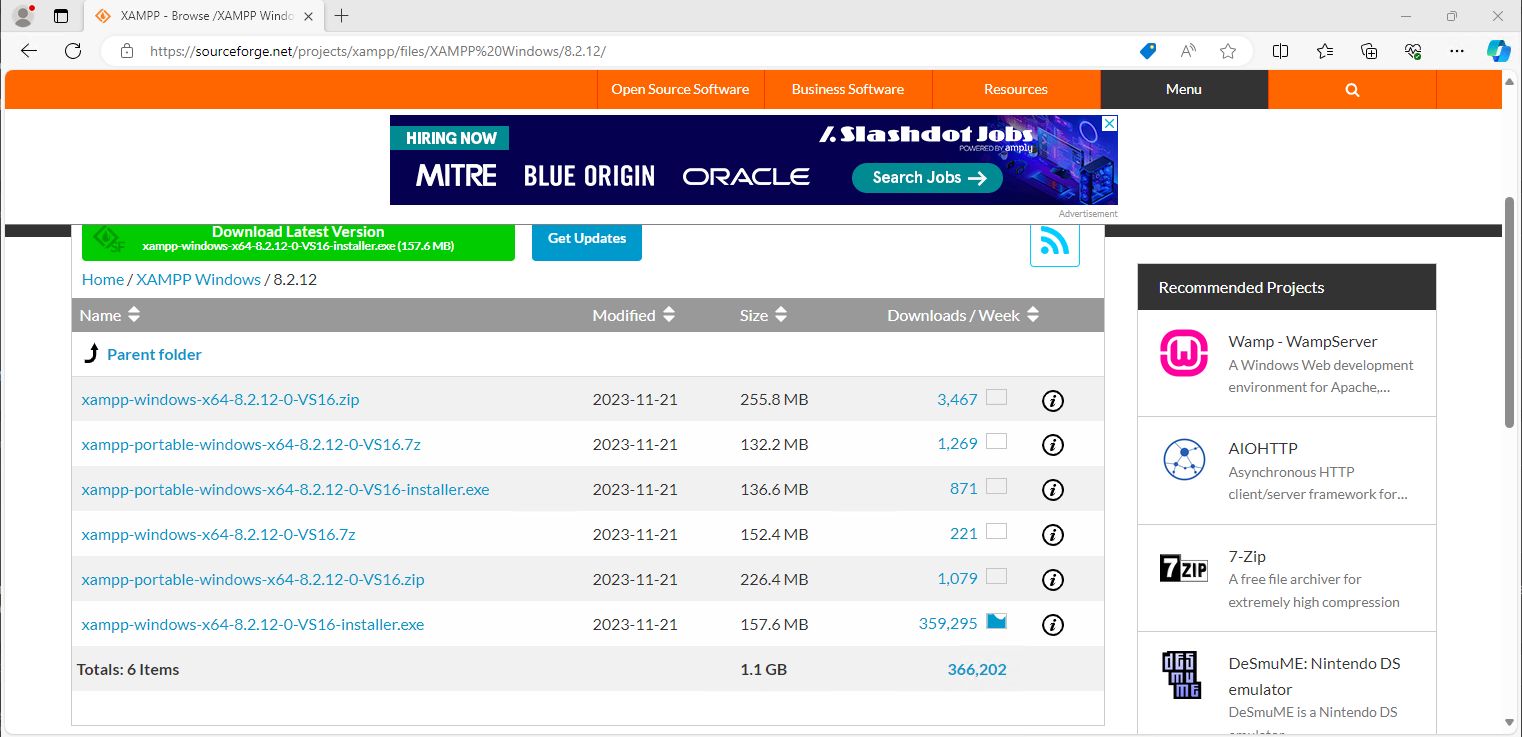
\includegraphics[scale=1.0]{xampp04} \\
            text & 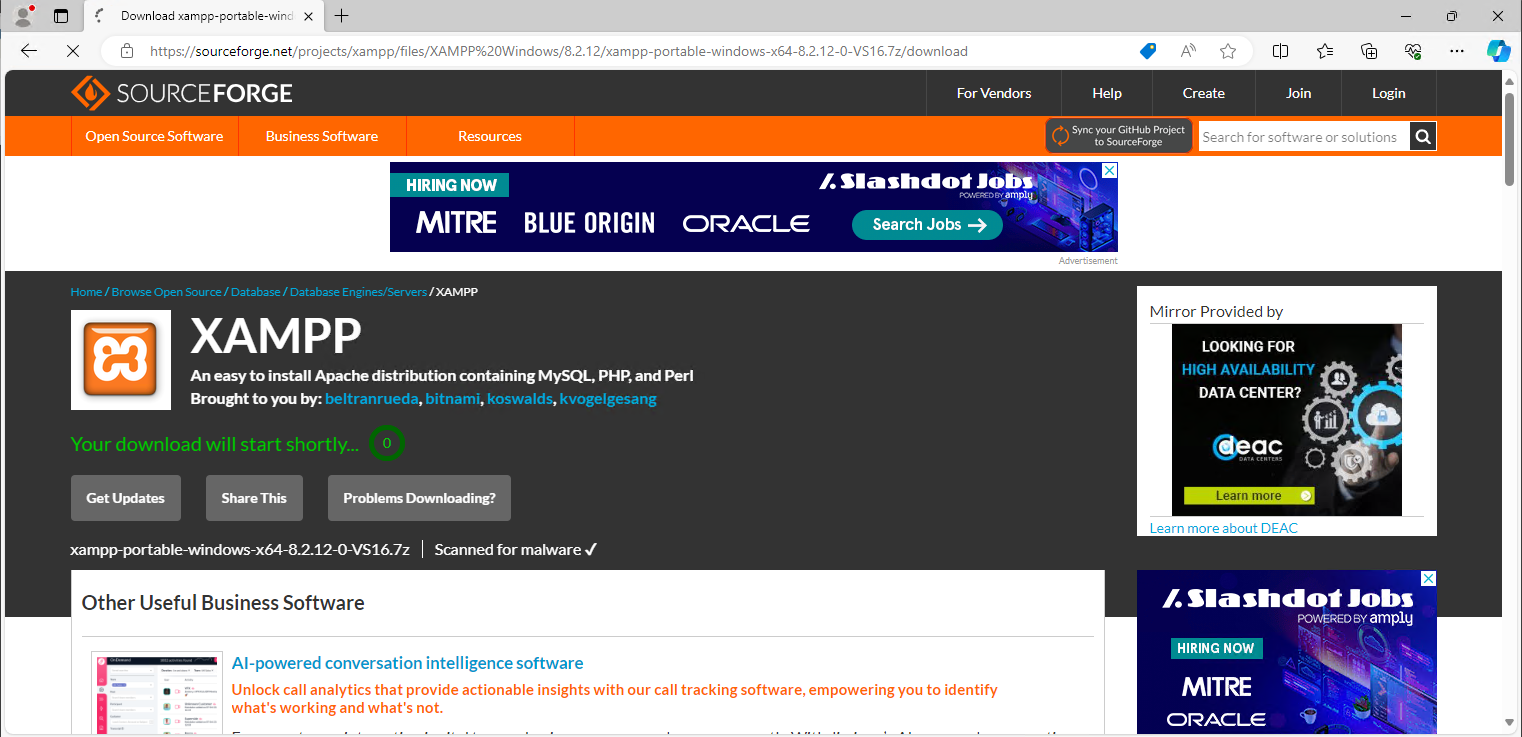
\includegraphics[scale=1.0]{xampp05} \\
            text & 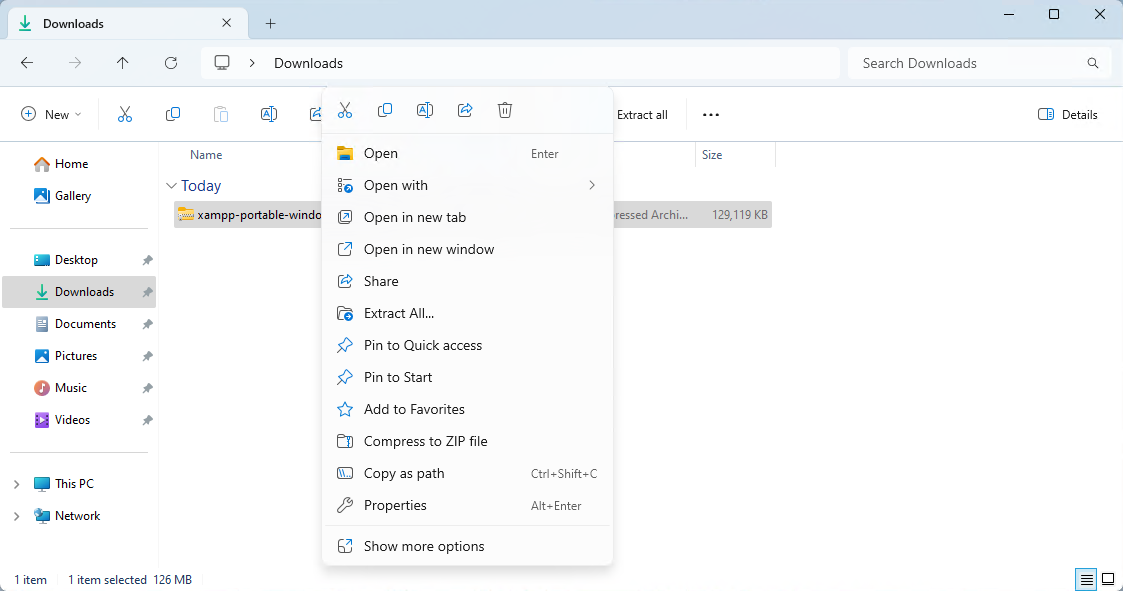
\includegraphics[scale=1.0]{xampp06} \\
            text & 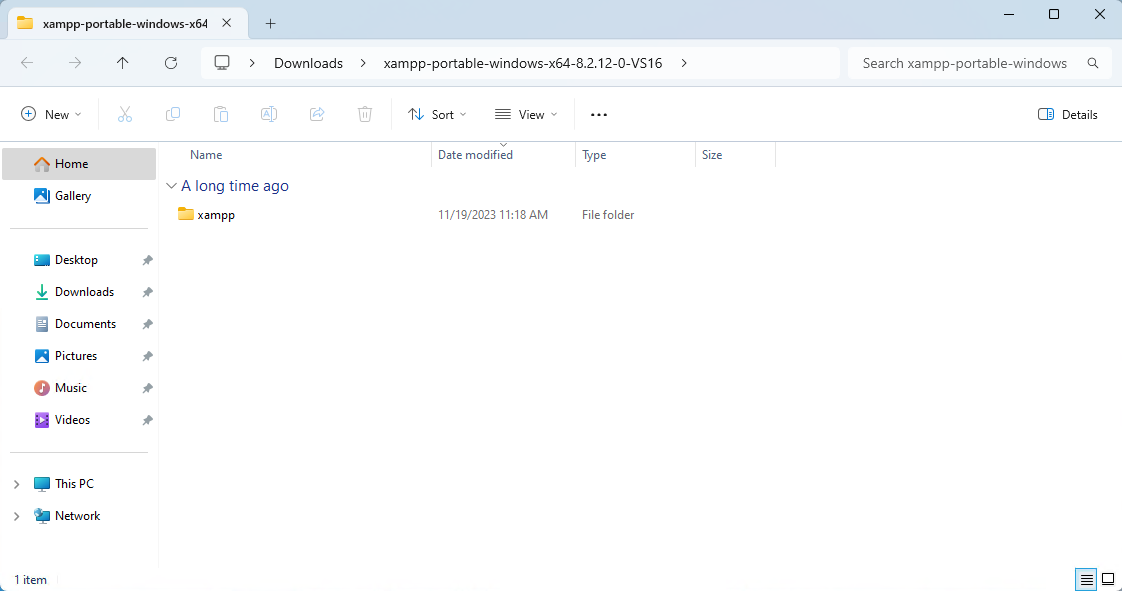
\includegraphics[scale=1.0]{xampp07} \\
            text & 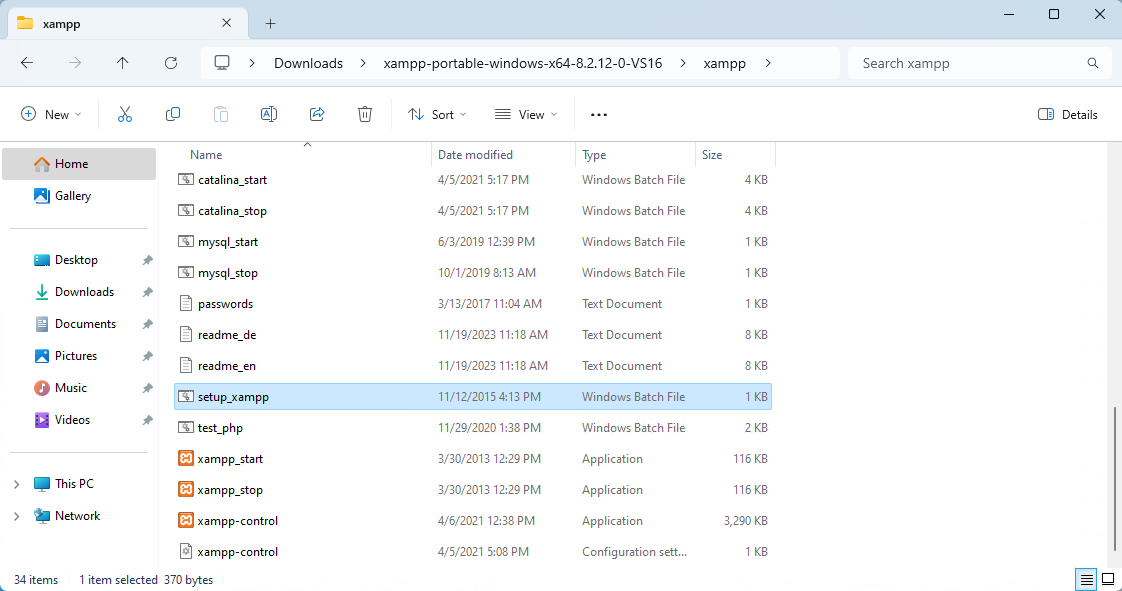
\includegraphics[scale=1.0]{xampp08} \\
            text & 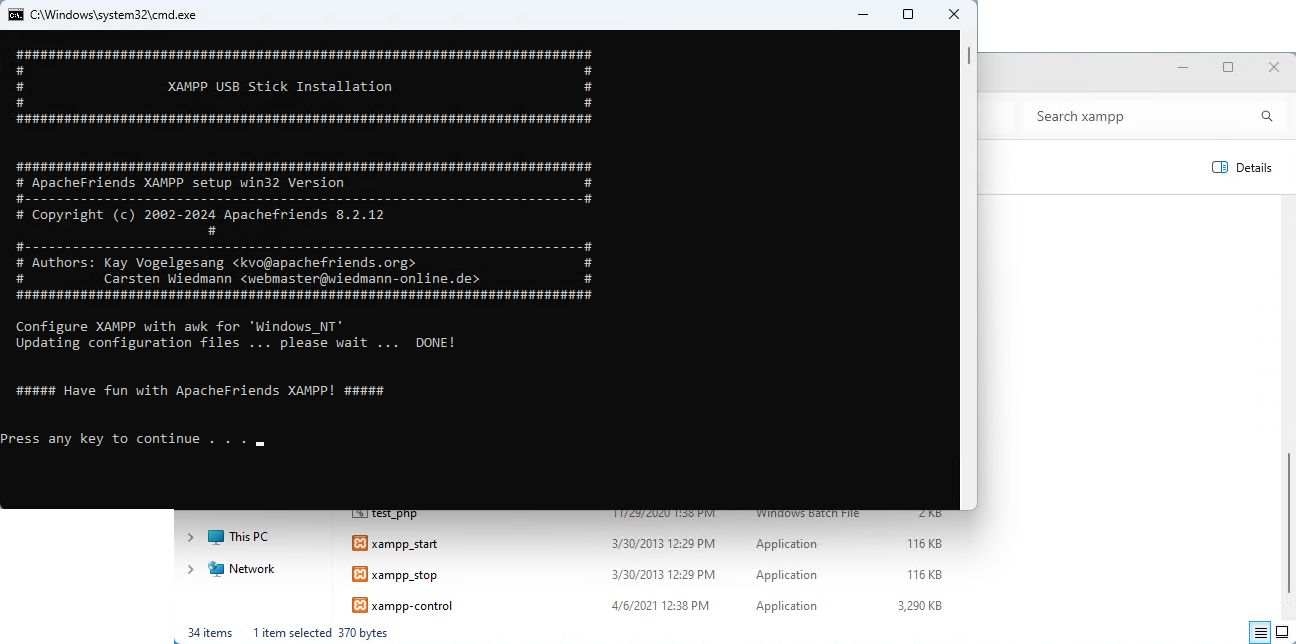
\includegraphics[scale=1.0]{xampp09} \\
            text & 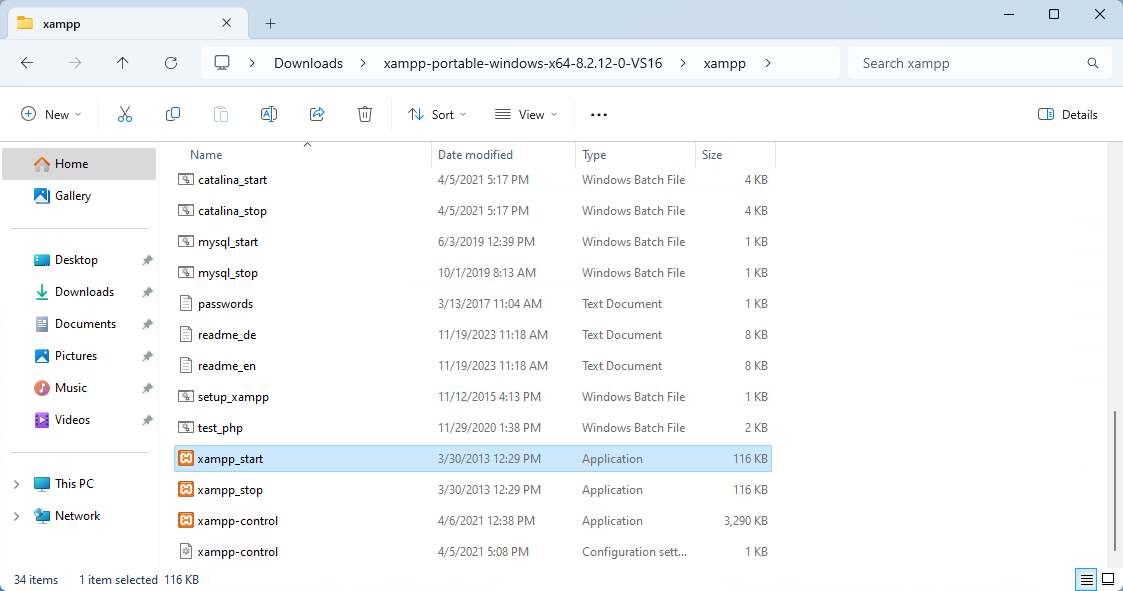
\includegraphics[scale=1.0]{xampp10} \\
            text & 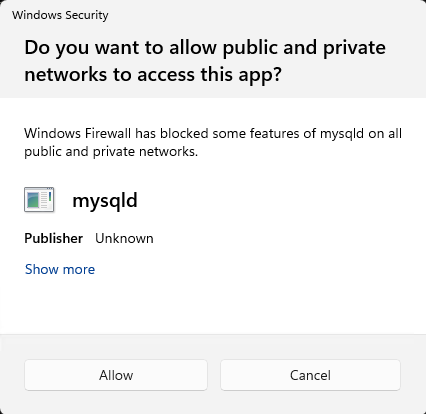
\includegraphics[scale=1.0]{xampp11} \\
            text & 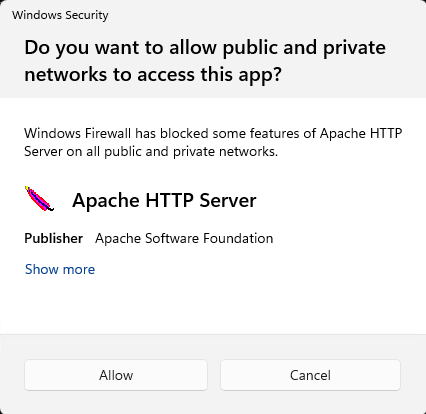
\includegraphics[scale=1.0]{xampp12} \\
            text & 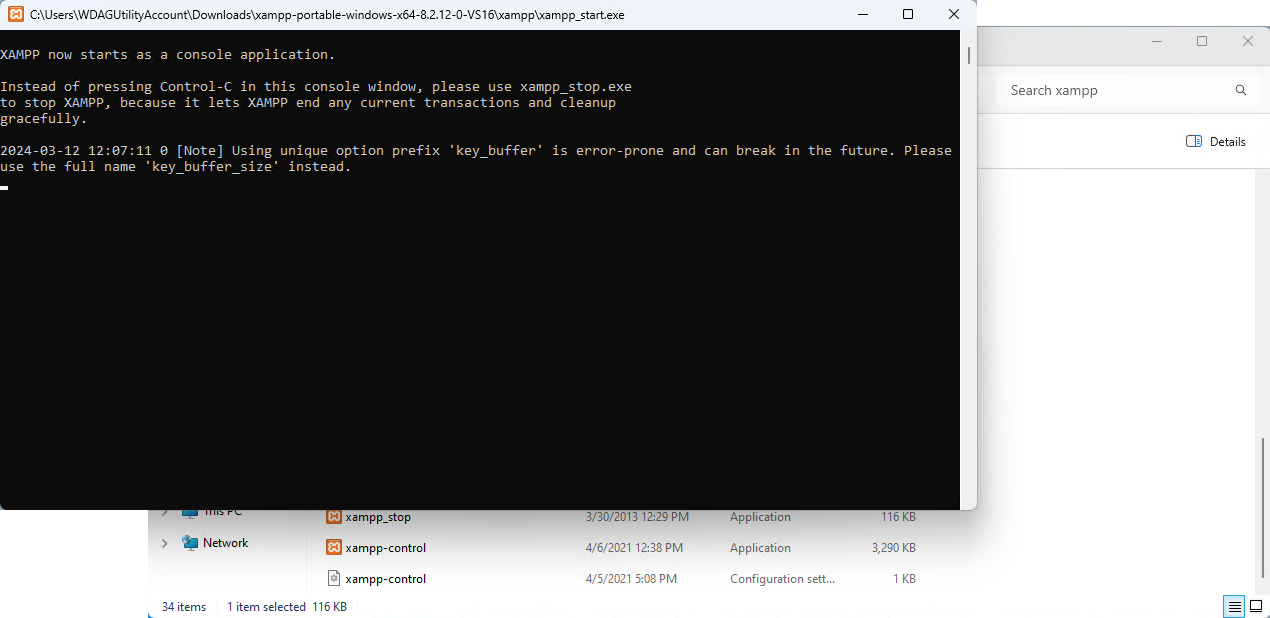
\includegraphics[scale=1.0]{xampp13} \\
            text & 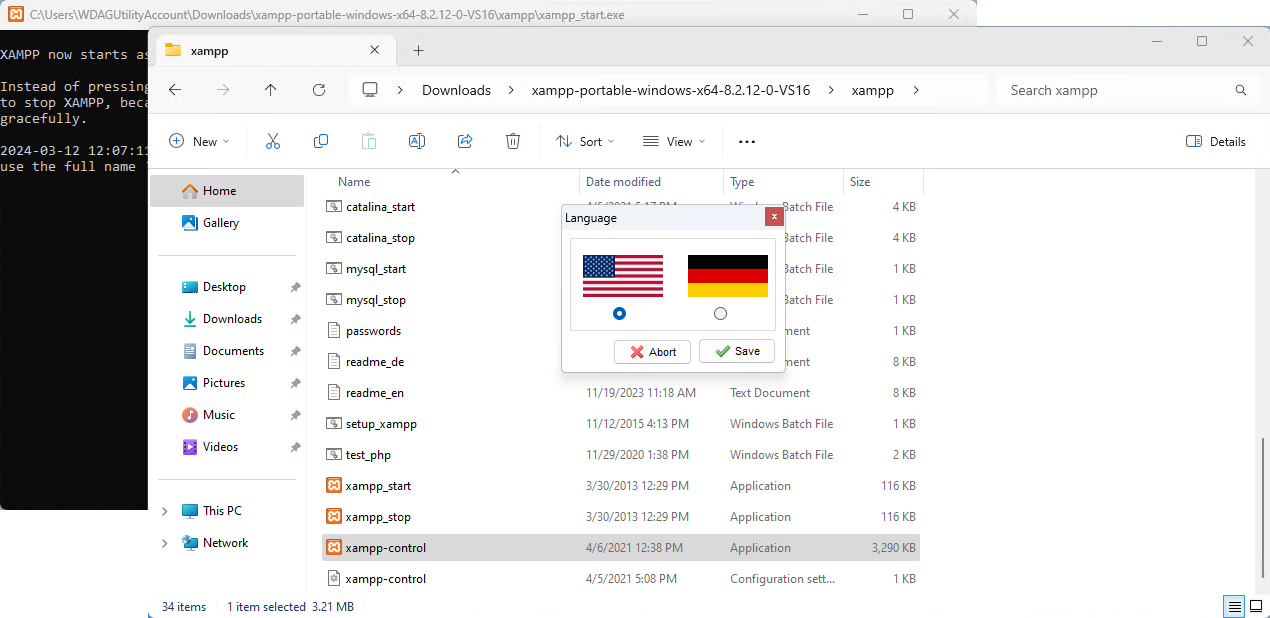
\includegraphics[scale=1.0]{xampp14} \\
            text & 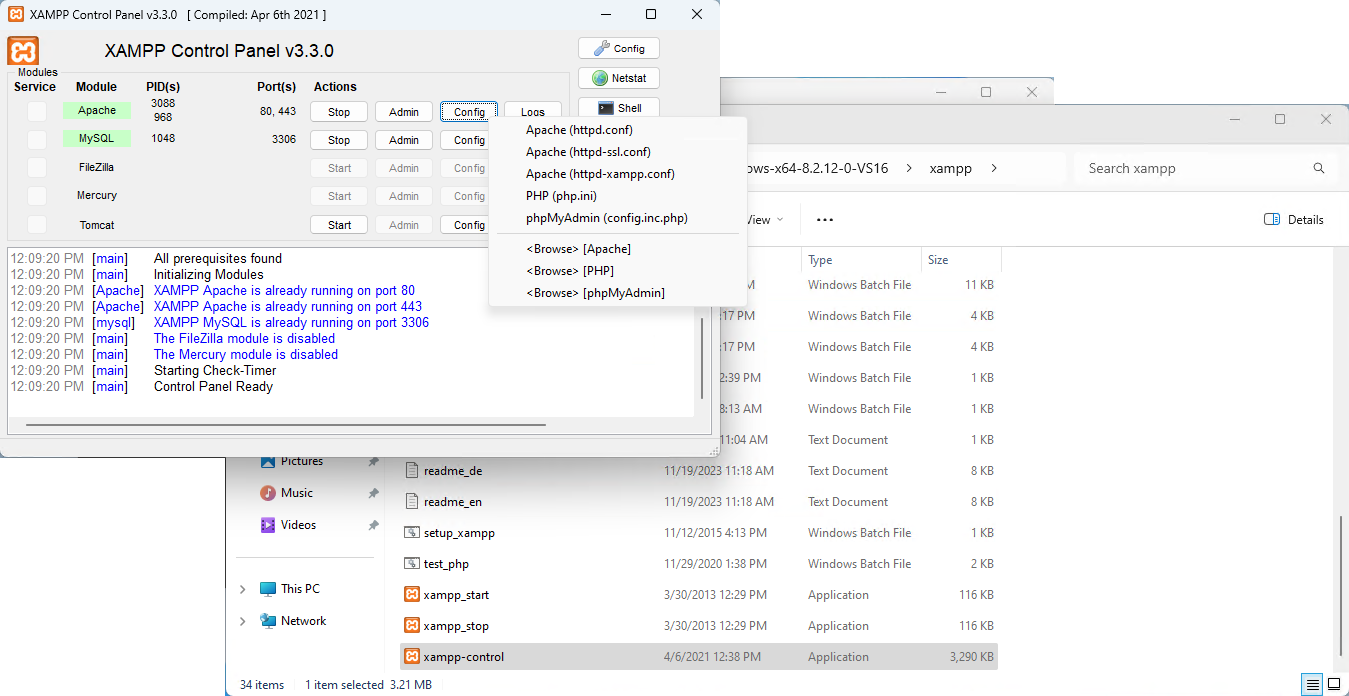
\includegraphics[scale=1.0]{xampp15} \\
            text & 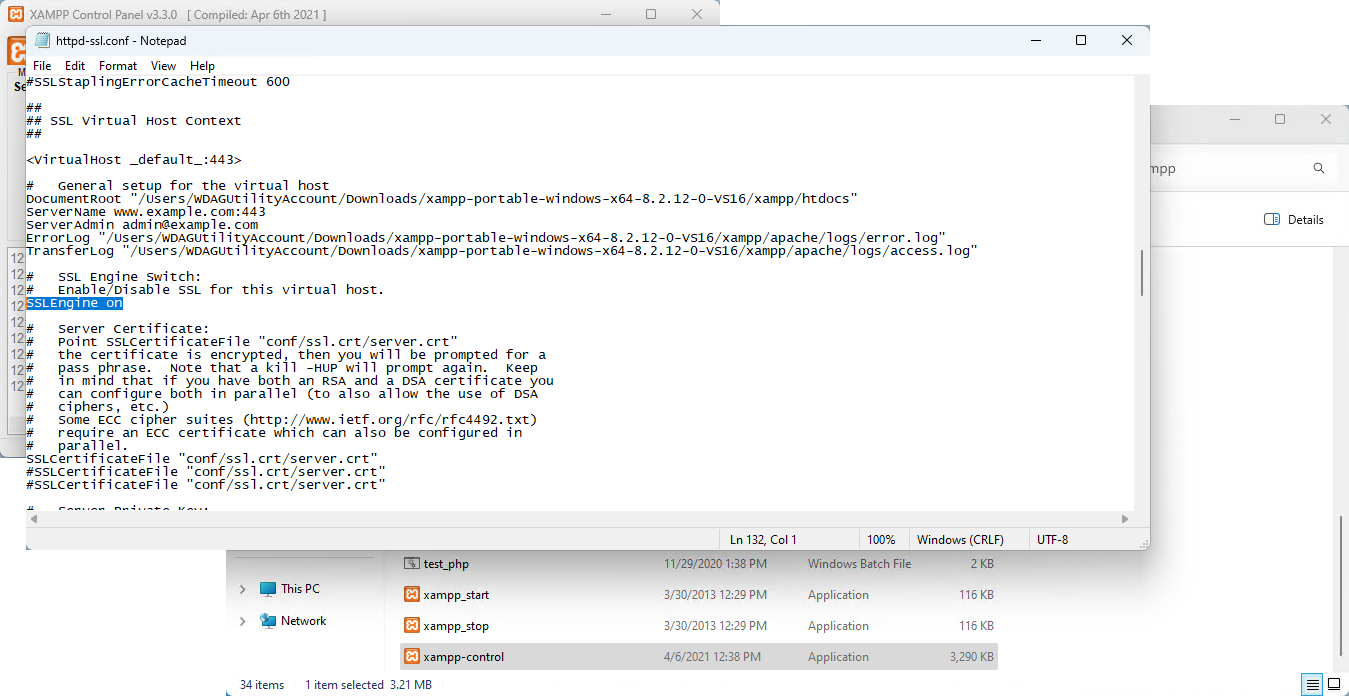
\includegraphics[scale=1.0]{xampp16} \\
            text & 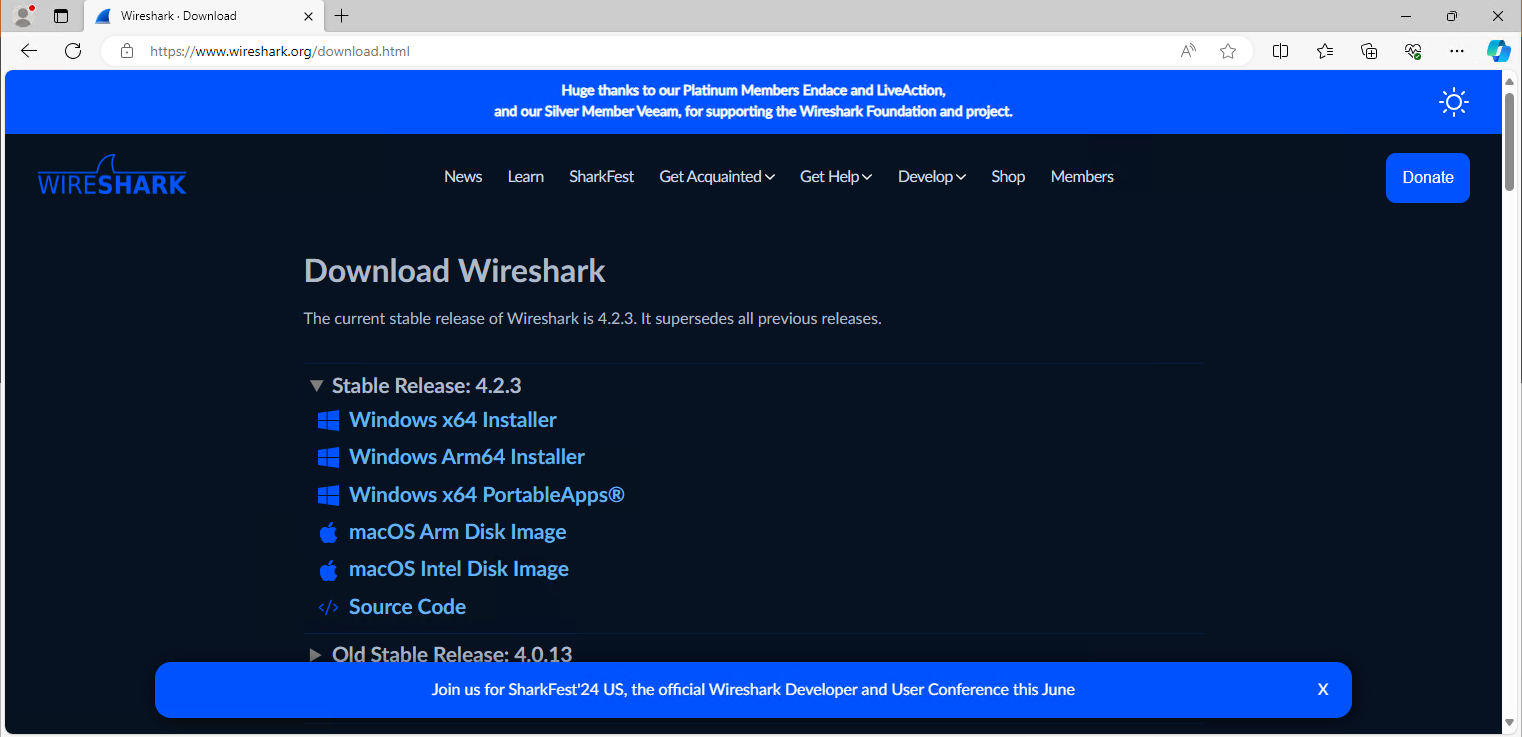
\includegraphics[scale=1.0]{wireshark01} \\
            text & 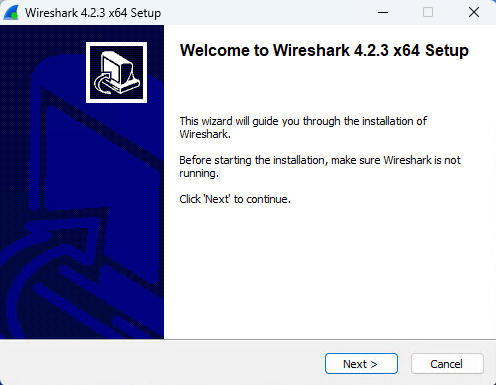
\includegraphics[scale=1.0]{wireshark02} \\
            text & 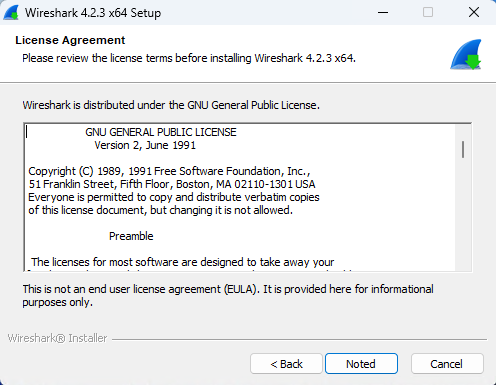
\includegraphics[scale=1.0]{wireshark03} \\
            text & 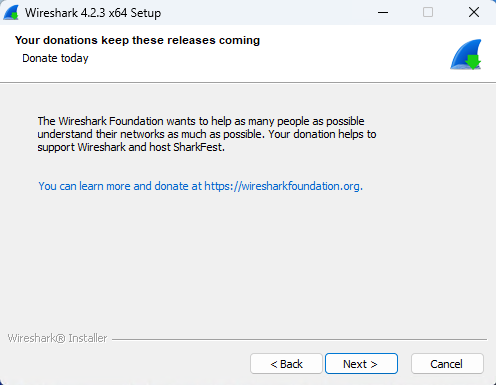
\includegraphics[scale=1.0]{wireshark04} \\
            text & 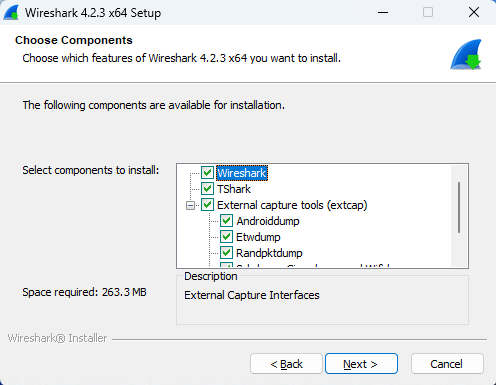
\includegraphics[scale=1.0]{wireshark05} \\
            text & 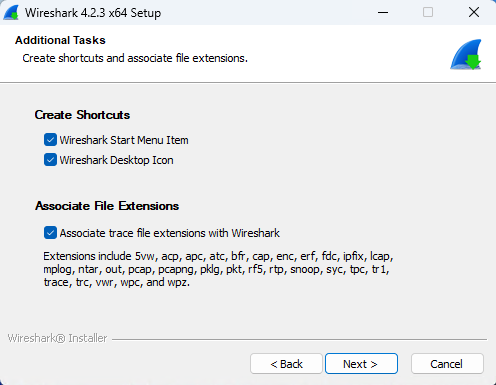
\includegraphics[scale=1.0]{wireshark06} \\
            text & 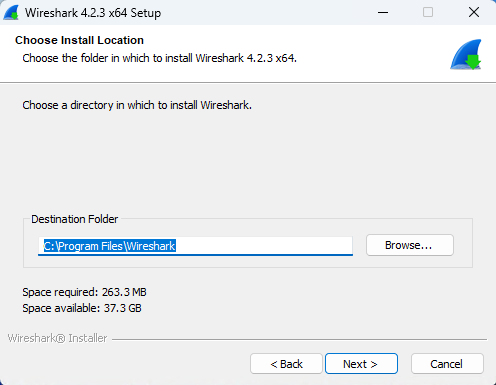
\includegraphics[scale=1.0]{wireshark07} \\
            text & 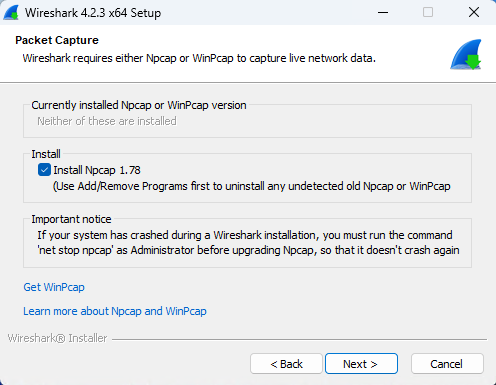
\includegraphics[scale=1.0]{wireshark08} \\
            text & 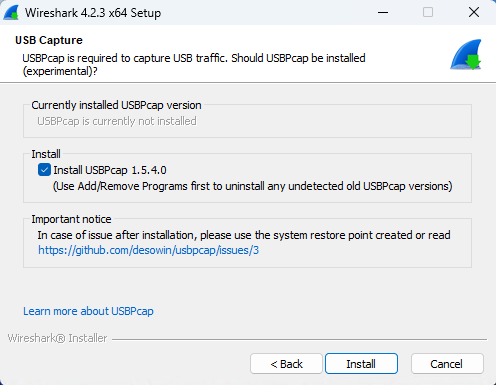
\includegraphics[scale=1.0]{wireshark09} \\
            text & 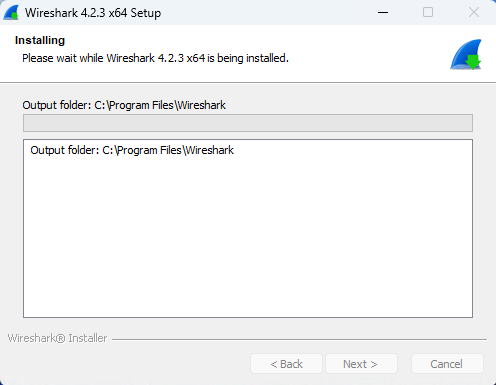
\includegraphics[scale=1.0]{wireshark10} \\
            text & 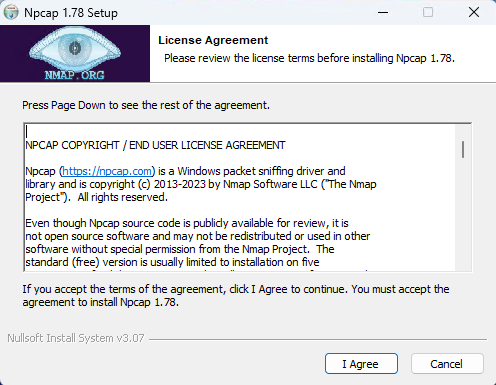
\includegraphics[scale=1.0]{wireshark11} \\
            text & 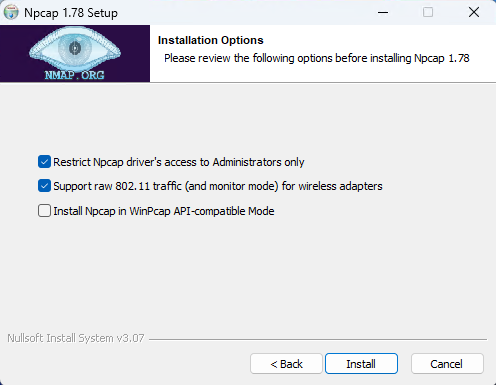
\includegraphics[scale=1.0]{wireshark12} \\
            text & 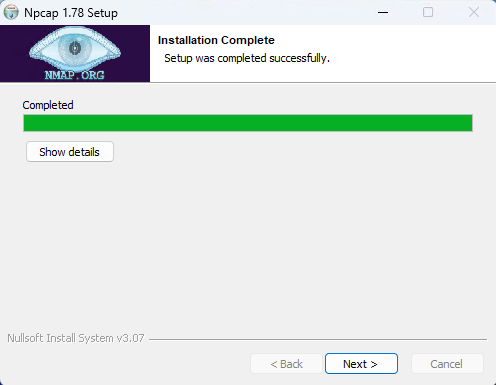
\includegraphics[scale=1.0]{wireshark13} \\
            text & 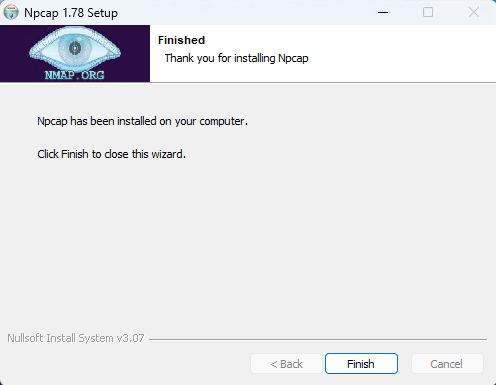
\includegraphics[scale=1.0]{wireshark14} \\
            text & 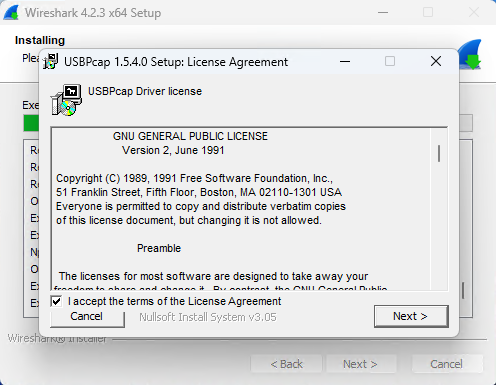
\includegraphics[scale=1.0]{wireshark15} \\
            text & 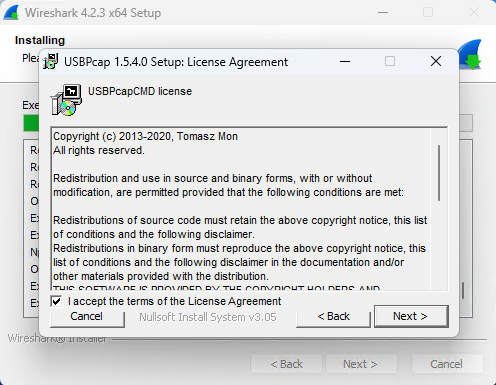
\includegraphics[scale=1.0]{wireshark16} \\
            text & 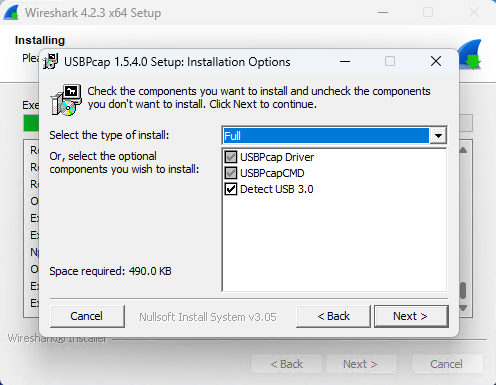
\includegraphics[scale=1.0]{wireshark17} \\
            text & 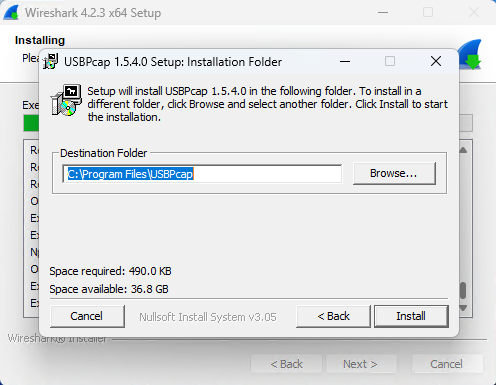
\includegraphics[scale=1.0]{wireshark18} \\
            text & 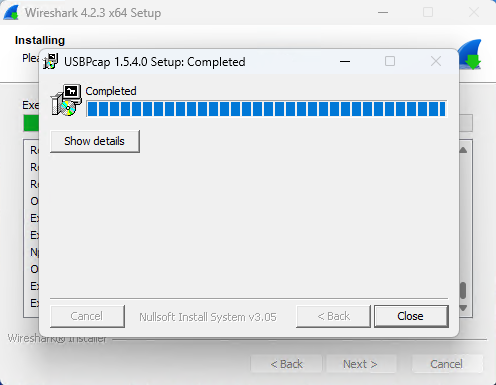
\includegraphics[scale=1.0]{wireshark19} \\
            text & 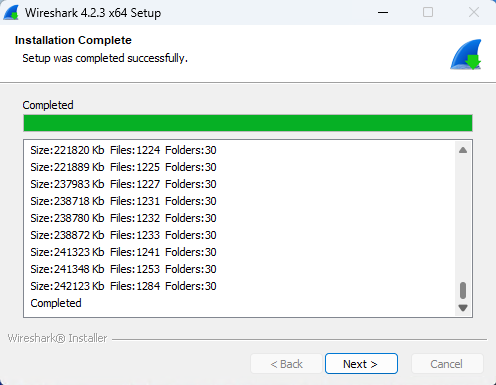
\includegraphics[scale=1.0]{wireshark20} \\
            text & 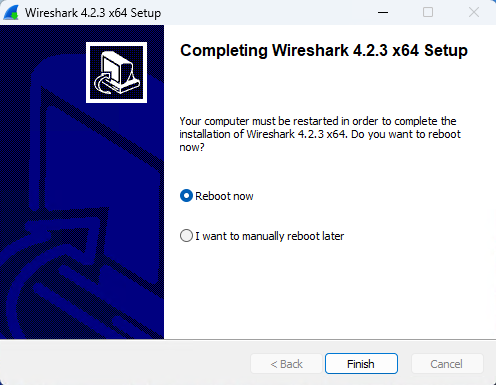
\includegraphics[scale=1.0]{wireshark21} \\
        \end{tabular}
        
        \begin{multicols}{2}
        [Install]
        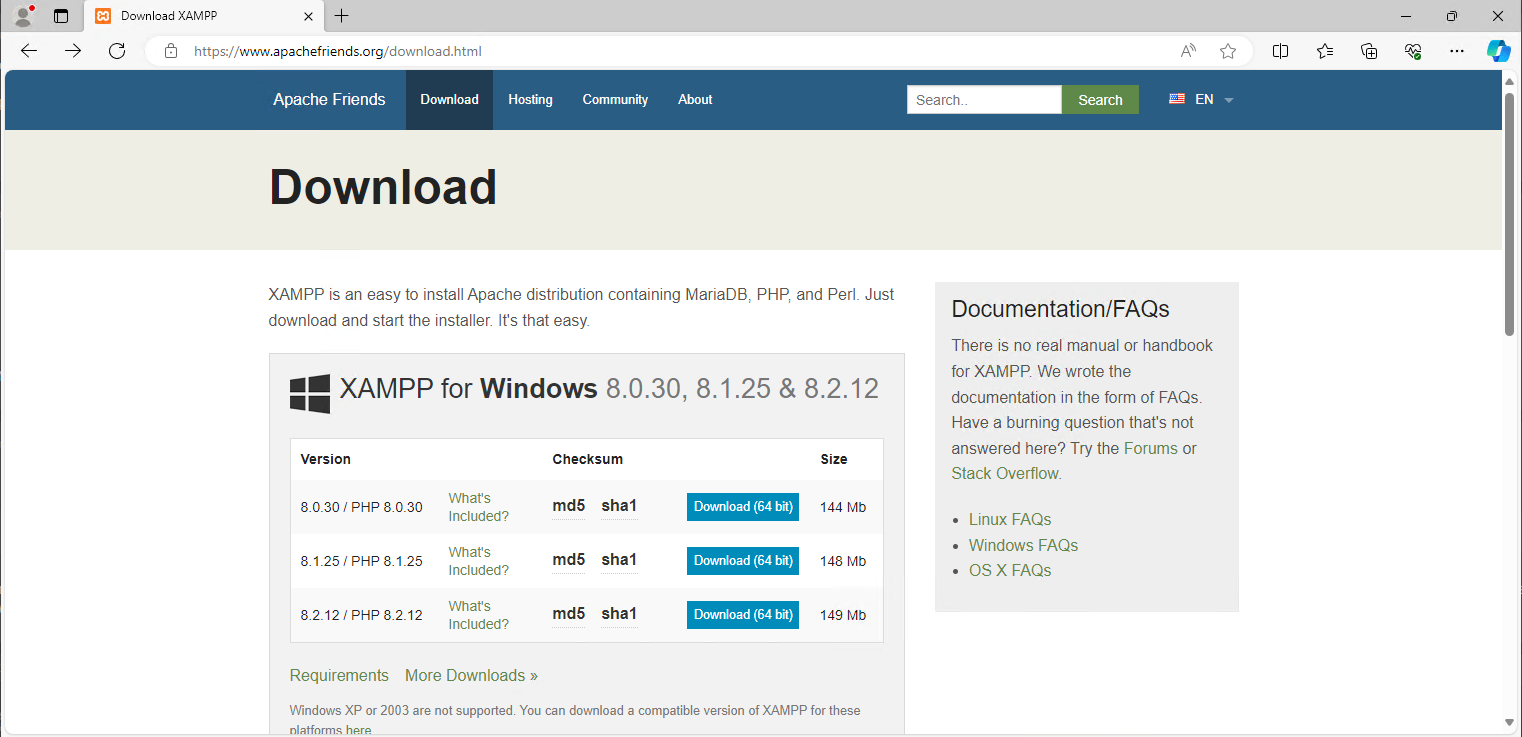
\includegraphics[scale=1.0]{1}

%% Chapter: recomendations -----------------------------------------------------{{{1
\section{Problems and resolutions}
    Python code: default system came with python2. Python3 installed.
    Encrypted html body: since the xampp server is running in a laptop at home and to make some progress i have to work remotely via vpn, the content came encrypted.
    Default http protocol SSL: disabled in apache2 the ssl engine

%% Chapter: conclusions --------------------------------------------------------{{{1

%% Bibliography ----------------------------------------------------------------{{{1

%% Appendix --------------------------------------------------------------------{{{1
%%1}}}

\end{document}
